\section{Hiện thực}
\subsection{Chức năng đã xây dựng}
\begin{itemize}
    \item Trang chủ: hiển thị sản phẩm mới nhất.
\item Danh mục sản phẩm, lọc theo category/size/price.
\item Tìm kiếm sản phẩm theo từ khóa.
\item Trang chi tiết sản phẩm.
\item Giỏ hàng với chức năng: thêm sản phẩm, cập nhật số lượng, xóa sản phẩm
\item Thanh toán cơ bản: chỉ định địa chỉ, số điện thoại, tạo hóa đơn đơn hàng
\item Đơn hàng: Theo dõi đơn hàng, lịch sử mua hàng, xác nhận đã nhận/hủy đơn, review sản phẩm.
\item Đăng ký/đăng nhập/đăng xuất.
\item Tin tức: danh sách và trang chi tiết.
\item Liên hệ: gửi thông tin liên hệ.
\item Admin: quản lý sản phẩm, quản lý danh mục. quản lý đơn hàng, quản lý người dùng, quản lý tin tức, quản lý phản hồi

\subsection{Cài đặt môi trường}
\begin{itemize}
    \item \textbf{Phần mềm:} XAMPP (PHP 7.4+), MySQL 5.7+.
    \item \textbf{Các bước cài đặt:}
    \begin{enumerate}
        \item Copy mã nguồn vào thư mục \texttt{xampp/htdocs/}.
        \item Import file \texttt{database.sql} thông qua phpMyAdmin.
        \item Cấu hình thông số kết nối ($host, db\_name, user, pass$) trong file \texttt{db.php}.
        \item Truy cập qua trình duyệt tại địa chỉ\\ \texttt{http://localhost/[folder\_name]/index.php}.
    \end{enumerate}
\end{itemize}


\subsection{Một số hình ảnh thực tế}
\begin{figure}[h!]
	\centering
	\includegraphics[width=\linewidth]{images/mainpage.png}
    \caption{Trang chủ}
\end{figure}

\begin{figure}[h!]
	\centering
	\includegraphics[width=\linewidth]{images/productlists.png}
    \caption{Trang sản phẩm}
\end{figure}
\begin{figure}[h!]
	\centering
	\includegraphics[width=\linewidth]{images/productdetail.png}
    \caption{Chi tiết sản phẩm}
\end{figure}
\begin{figure}[h!]
	\centering
	\includegraphics[width=\linewidth]{images/cart.png}
    \caption{Giỏ hàng}
\end{figure}

\begin{figure}[H]
	\centering
	\includegraphics[width=\linewidth]{images/xemdonhang.png}
    \caption{Xem lịch sử đơn hàng}
\end{figure}

\begin{figure}[H]
	\centering
	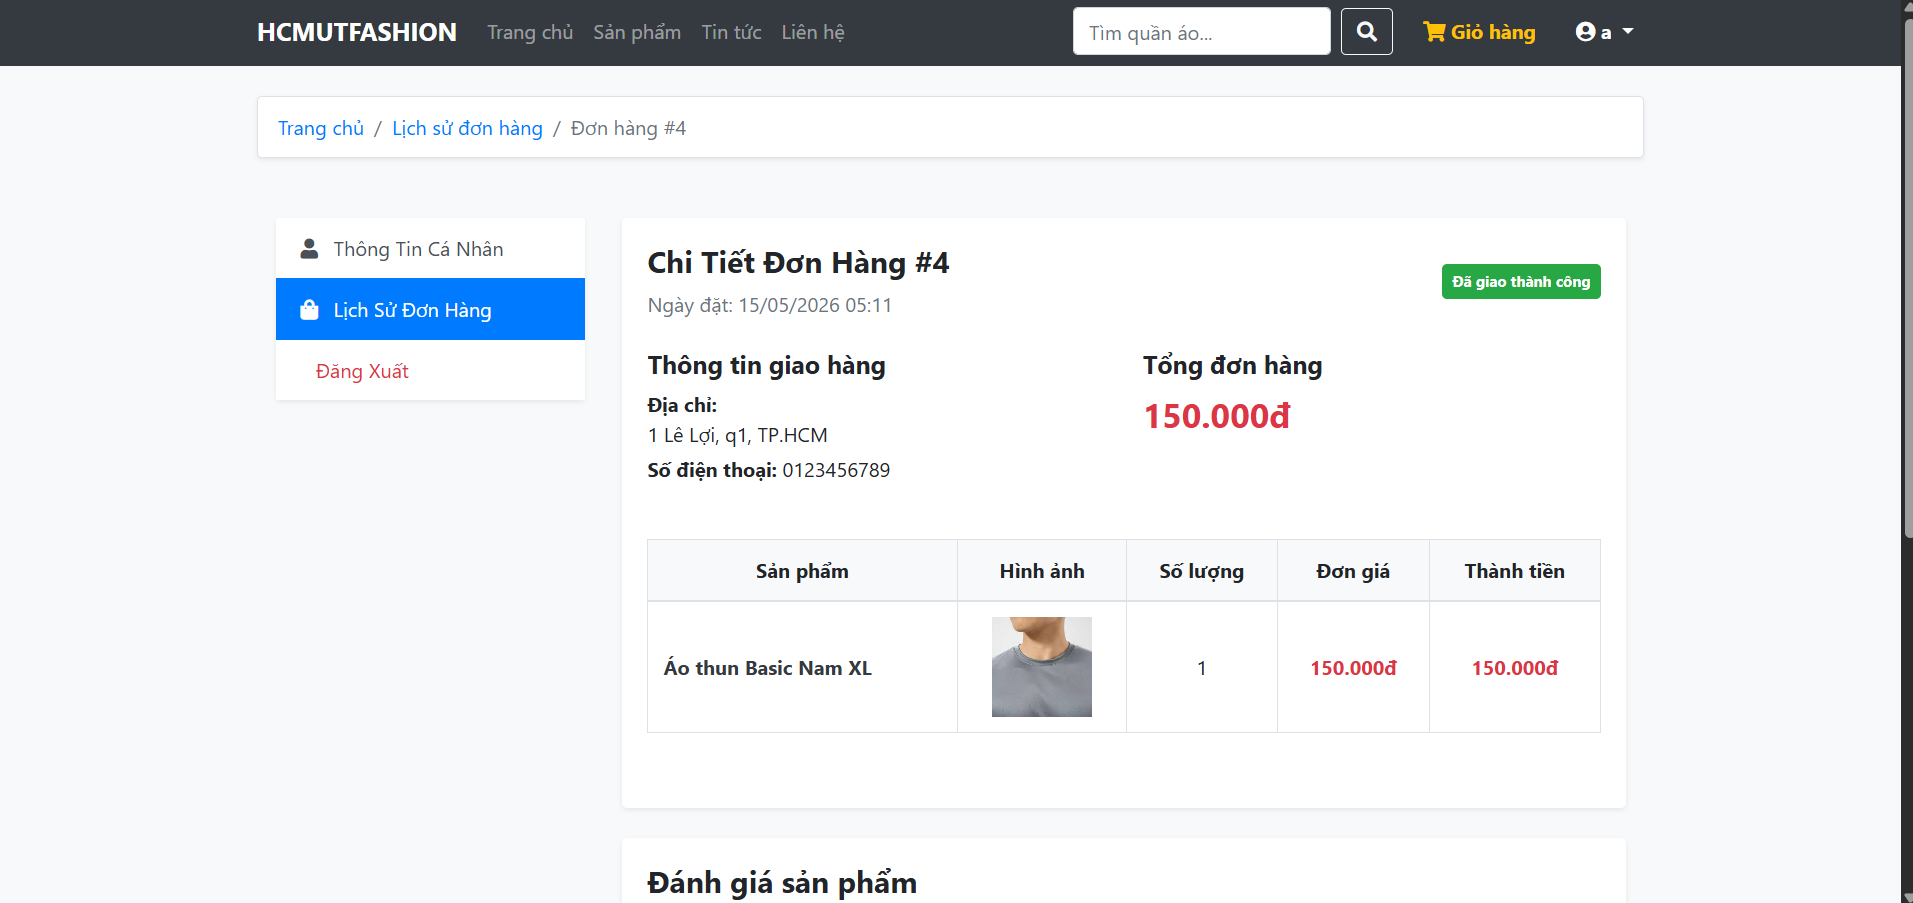
\includegraphics[width=\linewidth]{chapters/xemchitietdon.png}
    \caption{Xem chi tiết đơn hàng}
\end{figure}

\begin{figure}[h!]
	\centering
	\includegraphics[width=\linewidth]{images/adminpage.png}
    \caption{Trang dành riêng cho Admin sử dụng strdash}
\end{figure}
\end{itemize}
\newpage